\section{Experiments}
We now present the results of the three algorithm previously introduced: (i) Decentralized Stochastic Gradient Free Frank Wolfe, (ii) Decentralized Variance-Reduced Stochastic Gradient Free Frank Wolfe, (iii) Distributed Stochastic Gradient Free Frank Wolfe.\\
Our interest is to find a perturbation that is able to misclassify the MNIST digit images, keeping the image almost unchanged to the human eye. In order to generate an adversarial example we have to find $x'$ for a given input $x$ such that the corresponding loss function $L(x',y)$ is maximized, while still minimizing the $\ell_{\infty}$ norm related to it. This minimization is needed for keeping unchanged the vision of the digit. We set the constraint to be that of $\ell_{\infty}$ with $\varepsilon=0.25$. We perform the experimets on the MNIST dataset to find an universal adversarial perturbation, and we use the pretrained LeNet 5 model available from Pytorch to demonstrate the attacks.

\subsection{Decentralized Stochastic Gradient Free Frank Wolfe}
To study the performance of Algorithm \ref{decentralized} we use the 10000 images in the MNIST test set, after normalizing them. Since we are dealing with 784-dimensional images, the problem is high-dimesional. We split the digit images giving 10 samples for each class to our 10 workers. Doing so, make each worker holding a hundred images. After tuning the hyperparameter $m$ of the number of direction, we discovered that $m=15$ was the good compromise between the computation time and the overall results. For each image we estimated its gradient using 20, 50 and 100 queries.

\begin{figure}[htbp]
	\centering
	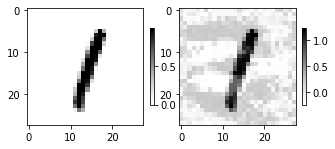
\includegraphics[width=3.8cm]{image_perturbation_example_30.png}\hfil
	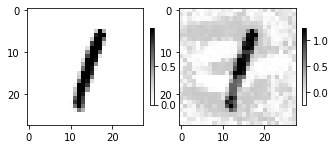
\includegraphics[width=3.8cm]{image_perturbation_example_35.png}
	\caption{Decentralized FW Perturbated Images: no clue on the parameters}
	\label{fig:decentralized}
\end{figure}
In Figure \ref{fig:decentralized} we can see an example of the perturbated images.

\subsection{Decentralized Variance-Reduced Stochastic Gradient Free Frank Wolfe}
For the Variance-Reduced FW algorithm we consider 5 workers and with 800 different images each, i.e. 160 images per digit. We set the number of queries to 20 and the number of component functions $S_2 = 3$. We then run the Algorithm \ref{variance-reduced} for $q=5,7,9$ and $n=5,10$. The choice for the values of $q$ is because of the different number of calling to the KWSA, while the $n$ parameter identify the different number of component function.\\
To quantify the performance of Algorithm \ref{variance-reduced}, it can be used the Frank-Wolfe duality gap, which is an upper bound on the primal suboptimality $f(x_t)-f(x^*)$, define as
\[ \mathcal{G} = \max_{v \in C} <F(x),x-v> \]
where $C$ is the associated constraint. In addition, it can also be used as a stopping criterion for FW algorithms.\\
From the theory we know that the major improvement of the variance reduction scheme is in terms of the fradient tracking performance, thath is, with $S_2 = (2d+9)\sqrt{n}/n_0$, $q = n_0 \sqrt{n}/6$, where $n_0 \in [1, \sqrt{n}/6)$. For the data that we have this tecnique for measuring the performances is unfeasible.\\

DA SPIEGARE MEGLIO, QUESTA PARTE NON L'AVEVO CAPITA MOLTO BENE :(

\subsection{Distributed Stochastic Gradient Free Frank Wolfe}
To test the performance of Algorithm \ref{distributed} we used 10 workers and an adjacecy matrix $A$ given by 
\[ A = 
\begin{pmatrix}
1& 1& 0& 1& 1& 1& 1& 1& 0& 1\\
1& 1& 1& 0& 1& 1& 1& 0& 1& 1\\
0& 1& 1& 1& 1& 1& 0& 1& 1& 1\\
1& 0& 1& 1& 1& 1& 0& 1& 1& 1\\
1& 1& 1& 1& 1& 1& 1& 0& 1& 1\\
1& 1& 1& 1& 1& 1& 1& 1& 1& 0\\
1& 1& 0& 0& 1& 1& 1& 1& 1& 1\\
1& 0& 1& 1& 0& 1& 1& 1& 1& 1\\
0& 1& 1& 1& 1& 1& 1& 1& 1& 1\\
1& 1& 1& 1& 1& 0& 1& 1& 1& 1	
\end{pmatrix}
.\]
We can notice that the diagonal is of ones, this because each node is connected to itself. Our network is composed of 10 nodes and the connectivity of the graph can be know by computing $\Vert W- J \Vert$, where $J= 11^T/10$ and $11^T$ represent a matrix with all entries set to 1. In our case we have a connectivity value of 0.438. We use 15 directions and test the algorithm for 20, 50 and 100 queries.

\begin{figure}[htbp]
	\centering
	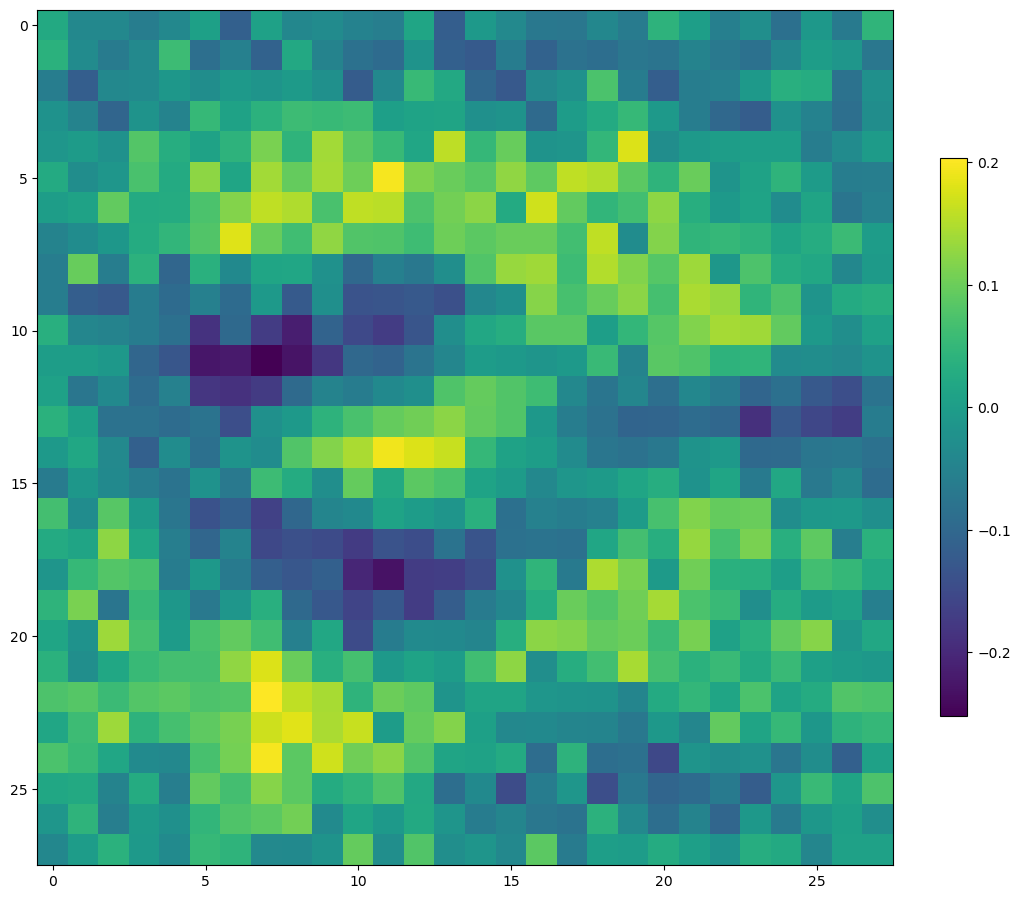
\includegraphics[width=3cm]{report_distributed_delta_100_15.png}\hfil
	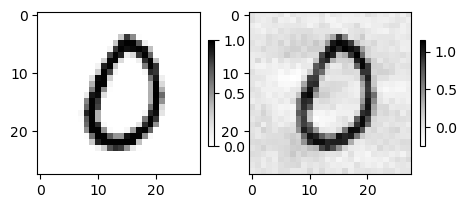
\includegraphics[width=5cm]{report_perturbated_img_100_15.png}
	\caption{Perturbation and perturbed image of the distributed FW with T=100 and m=15.}
	\label{fig:distributed_delta_50+20}
\end{figure}
In Figure \ref{fig:distributed_delta_50+20} we can see an example of the perturbations.
\subsection{Comparison between the perturbations}
